\documentclass[11pt]{amsart}

\usepackage[T1]{fontenc}
\usepackage{lmodern}
\usepackage{amssymb,amsmath}
\usepackage{graphicx}
\usepackage{booktabs}
\usepackage{enumitem}
\usepackage[dvipsnames]{xcolor}
\usepackage[margin=1.15in]{geometry}
\usepackage{microtype}
\usepackage{xurl}
\usepackage[colorlinks=true,linkcolor=blue!50!black,citecolor=blue!50!black,urlcolor=blue!50!black]{hyperref}
\emergencystretch=3em

\newtheorem{theorem}{Theorem}[section]
\newtheorem{proposition}[theorem]{Proposition}
\newtheorem{lemma}[theorem]{Lemma}
\newtheorem{corollary}[theorem]{Corollary}
\newtheorem{introthm}{Theorem}
\newtheorem{introcor}[introthm]{Corollary}
\theoremstyle{definition}
\newtheorem{definition}[theorem]{Definition}
\theoremstyle{remark}
\newtheorem{remark}[theorem]{Remark}
\numberwithin{equation}{section}

\renewcommand{\Re}{\operatorname{Re}}
\renewcommand{\Im}{\operatorname{Im}}
\newcommand{\Lam}{\Lambda_\chi}
\newcommand{\Q}{\mathbb{Q}}
\newcommand{\Z}{\mathbb{Z}}
\newcommand{\fp}{\mathfrak{p}}
\newcommand{\Hyp}{\mathrm{H}}
\DeclareMathOperator{\Cl}{Cl}
\providecommand{\doi}[1]{\href{https://doi.org/#1}{doi:\nolinkurl{#1}}}
\hypersetup{pdftitle={Split Primes and the Exponent of Imaginary Quadratic Class Groups},pdfauthor={Deep Bhattacharjee}}

\begin{document}

\title{Split Primes and the Exponent of Imaginary Quadratic Class Groups}

\author{Deep Bhattacharjee}
\address{Formerly, Electro-Gravitational Space Propulsion Laboratory (EGSPL),\newline Bhubaneswar, Odisha 751030, India\newline
Formerly, University of Calcutta (Heramba Chandra College),\newline 23/49 Gariahat Road, Golpark, Kolkata 700029, West Bengal, India}
\email{d.bhattacharjee@erl-forschung.de}
\email{itsdeep@live.com}
\email{egspl@proton.me}
\urladdr{https://orcid.org/0000-0003-0466-750X}
\urladdr{https://github.com/creelie}
\thanks{Corresponding author: Deep Bhattacharjee, \href{mailto:d.bhattacharjee@erl-forschung.de}{d.bhattacharjee@erl-forschung.de}; ORCID \href{https://orcid.org/0000-0003-0466-750X}{\mbox{0000-0003-0466-750X}}. For the code and data: \href{mailto:egspl@proton.me}{egspl@proton.me} (GitHub: creelie).}

\subjclass[2020]{11R29, 11R11, 11M20, 11E16, 11Y40}
\keywords{imaginary quadratic fields, class group exponent, split primes, idoneal numbers, zero-free half-plane}

\begin{abstract}
Assume that no Dirichlet $L$-function vanishes in the half-plane $\Re s>11/12$, as a recent preprint asserts. Then every imaginary quadratic field $\Q(\sqrt d)$ has a split prime below $(2\log|d|)^{12}$, its class group has exponent at least $\log(|d|/4)/(12\log(2\log|d|))$, and Euler's sixty-five idoneal numbers are all of them. With $\Re s>7/8$ the exponent $12$ becomes $8$.
\end{abstract}

\maketitle

\section{Introduction}\label{sec:intro}

Let $d<0$ be a fundamental discriminant, $K=\Q(\sqrt d)$, and let $E(d)$ be the exponent of the class group $\Cl(d)$ of $K$. Chowla \cite{Cho34} proved that only finitely many imaginary quadratic fields have a class group that is an elementary abelian $2$-group, that is, $E(d)\le2$; the proof is ineffective because of a possible Siegel zero. Under the generalised Riemann hypothesis, Boyd and Kisilevsky \cite{BK72} and Weinberger \cite{Wei73} showed $E(d)\gg\log|d|/\log\log|d|$; without any hypothesis it is not known that $E(d)\to\infty$ \cite{EKN20}. Weinberger also showed that at most one field with $|d|>5460$ has $E(d)\le2$, and none under the generalised Riemann hypothesis. Heath-Brown \cite{HB08} proved finiteness for the exponents $5$, $2^r$ and $3\cdot2^r$ (see also Earnest and K\"orner \cite{EK82}), and Elsenhans, Kl\"uners and Nicolae \cite{EKN20} computed all fields with $E(d)\le 8$ and $|d|\le 3.1\cdot10^{20}$ and showed that their lists for $E(d)\in\{2,4,8\}$ are complete if no $L(s,\chi_d)$ has a real zero close to $s=1$.\footnote{Their condition is that $L(s,\chi_d)\neq0$ for $1-1/(4\log|d|)\le s<1$ whenever $|d|>e^{11.2}$; it rests on Tatuzawa's explicit form of Siegel's theorem.}

All these results pass through one elementary observation. If a prime $p$ splits in $K$ as $p\mathcal O_K=\fp\bar\fp$ and $p^c<|d|/4$, then $\fp^c$ is not principal (Lemma~\ref{lem:order}). A split prime of size $(\log|d|)^{O(1)}$ therefore forces $E(d)\gg\log|d|/\log\log|d|$. Under the generalised Riemann hypothesis such a prime, of size $O(\log^2|d|)$, comes from the method of Ankeny \cite{Ank52}, which Bach made explicit \cite{Bac90}.

A zero-free half-plane is enough to replace the generalised Riemann hypothesis here. For $\tfrac12\le B<1$ write
\[
\Hyp(B):\qquad L(s,\chi)\neq0\quad\text{for every primitive Dirichlet character }\chi\text{ and every }s\text{ with }\Re s>B .
\]
Two recent preprints of OpenAI assert $\Hyp(7/8)$ \cite{OAI-a} and $\Hyp(11/12)$ \cite{OAI-b}; a third excludes Landau--Siegel zeros uniformly \cite{OAI-c}. These preprints have not been refereed. Every theorem below states the hypothesis it uses, and $\Hyp(7/8)$ implies $\Hyp(11/12)$.\footnote{The three preprints are dated 30 September, 5 October and 1 October 2026 and are kept in the repository \url{https://github.com/openai/math}.}

\begin{introthm}\label{thm:A}
Assume $\Hyp(11/12)$. Every imaginary quadratic field $\Q(\sqrt d)$ has a prime $p\le(2\log|d|)^{12}$ that splits in it. Under $\Hyp(7/8)$ the same holds with $p\le(2\log|d|)^8$.
\end{introthm}

Under $\Hyp(B)$ the argument gives a split prime of size $(c\log|d|)^{1/(1-B)}$; the work lies in making $c$ explicit and small and in covering all $d$ at once, which Proposition~\ref{prop:criterion} and Section~\ref{sec:proofA} do with $c=2$.\footnote{The qualitative form, a prime with $\chi(p)=1$ below a power of $\log q$ under a zero-free half-plane, is a classical consequence of the explicit formula. The preprint \cite{OAI-b} records the analogous consequence for the least quadratic non-residue.}

\begin{introthm}\label{thm:B}
Assume $\Hyp(7/8)$. Every fundamental discriminant $d<-4$ satisfies
\[
E(d)\ \ge\ \frac{\log(|d|/4)}{8\log(2\log|d|)} .
\]
Consequently every field with $E(d)\le e$ has $|d|\le N_e$, where $\log_{10}N_e$ is given in Table~\ref{tab:Ne}. Under $\Hyp(11/12)$ the same holds with $12$ in place of $8$ and the second row of the table.
\end{introthm}

\begin{table}[ht]
\centering
\caption{Upper bounds $\log_{10}N_e$ for $|d|$ when $E(d)\le e$.}\label{tab:Ne}
\begin{tabular}{@{}lccccccccc@{}}
\toprule
$e$ & $2$ & $3$ & $4$ & $5$ & $6$ & $7$ & $8$ & $9$ & $10$\\
\midrule
$\Hyp(7/8)$ & $36.15$ & $59.03$ & $83.29$ & $108.57$ & $134.65$ & $161.39$ & $188.71$ & $216.52$ & $244.77$\\
$\Hyp(11/12)$ & $59.03$ & $95.82$ & $134.65$ & $174.99$ & $216.52$ & $259.05$ & $302.42$ & $346.53$ & $391.30$\\
\bottomrule
\end{tabular}
\end{table}

The order $\log|d|/\log\log|d|$ is the one obtained from the generalised Riemann hypothesis; the half-plane only costs the factor $1-B$ in the constant. For $e=7$ even the finiteness of the set of fields with $E(d)=7$ was not known without hypothesis \cite{EKN20}. Under $\Hyp(11/12)$ the computation of Elsenhans, Kl\"uners and Nicolae becomes unconditional for $E(d)\in\{2,4,8\}$ (Remark~\ref{rem:EKN}).

For exponent two we give a self-contained proof of the complete list. Let $D<0$ be any discriminant and $C(D)$ the group of classes of primitive positive definite binary quadratic forms of discriminant $D$.

\begin{introthm}\label{thm:C}
Assume $\Hyp(11/12)$. Exactly $101$ negative discriminants $D$ have $C(D)$ of exponent at most $2$. The largest is $|D|=7392$; exactly $65$ of them are fundamental, the largest being $|d|=5460$. They are listed in Appendix~\ref{app:list}.
\end{introthm}

A positive integer $n$ is idoneal (Euler's \emph{numerus idoneus}) if, roughly, every odd number properly represented by $x^2+ny^2$ in only one way is prime; by Grube's theorem $n$ is idoneal if and only if every genus of forms of discriminant $-4n$ consists of a single class \cite{Kan11}, \cite[Theorem 3.22 and Proposition 3.24]{Cox13}. Euler found $65$ idoneal numbers, and without a hypothesis on zeros it is not known that there are no others \cite{Kan11}.

\begin{introcor}\label{cor:idoneal}
Assume $\Hyp(11/12)$. The idoneal numbers are exactly
$1$, $2$, $3$, $4$, $5$, $6$, $7$, $8$, $9$, $10$, $12$, $13$, $15$, $16$, $18$, $21$, $22$, $24$, $25$, $28$, $30$, $33$, $37$, $40$, $42$, $45$, $48$, $57$, $58$, $60$, $70$, $72$, $78$, $85$, $88$, $93$, $102$, $105$, $112$, $120$, $130$, $133$, $165$, $168$, $177$, $190$, $210$, $232$, $240$, $253$, $273$, $280$, $312$, $330$, $345$, $357$, $385$, $408$, $462$, $520$, $760$, $840$, $1320$, $1365$, $1848$.
\end{introcor}

The completeness of Euler's list under $\Hyp(11/12)$ was observed in \cite{OAI-b}, by combining the computation of \cite{EKN20} with Grube's reduction to fundamental discriminants. The proof given here is independent of both: it combines the lower bound $h(d)\ge 7612$ for $|d|>2^{40}$ (Corollary~\ref{cor:h}), a sieve over $10^6<|d|\le2^{40}$ by Lemma~\ref{lem:order}, a direct count of reduced forms for $|D|\le10^6$, and an arithmetic reduction of non-fundamental discriminants to fundamental ones (Section~\ref{sec:two}).

\subsection*{Method}
Theorem~\ref{thm:A} is proved with an explicit formula whose weight is a triangle in $\log n$ of half-width $L$ centred at $\log y$ (Lemma~\ref{lem:triangle}). If no prime up to $ye^L$ splits, the prime side is close to $-y$. Under $\Hyp(B)$ each zero contributes at most $y^B$ times a quantity controlled by the Hadamard product, and the sum over zeros is $O(y^B\log q)$. The choice $y\asymp(\log q)^{1/(1-B)}$ balances the two, and the inequalities of Rosser and Schoenfeld \cite{RS62} make every constant explicit. Theorem~\ref{thm:C} needs a lower bound for $L(1,\chi_d)$ instead, and Section~\ref{sec:L1} proves one by integrating a second explicit formula along the ray $s=1+u$, in the spirit of Littlewood \cite{Lit28}. All constants are certified in ball arithmetic \cite{Joh17}.

\subsection*{Organisation}
Section~\ref{sec:prelim} collects the lemmas on split primes and forms. Section~\ref{sec:explicit} proves the explicit formulas and bounds the zeros. Section~\ref{sec:proofA} proves Theorems~\ref{thm:A} and~\ref{thm:B}, Section~\ref{sec:L1} the lower bound for $L(1,\chi)$, and Section~\ref{sec:two} Theorem~\ref{thm:C}. Appendix~\ref{app:contour} contains the contour shifts, Appendix~\ref{app:numerics} the certified constants, Appendix~\ref{app:list} the list of Theorem~\ref{thm:C}.

\section{Split primes, ideal classes and forms}\label{sec:prelim}

Throughout, $d<0$ is a fundamental discriminant, $K=\Q(\sqrt d)$, $\chi_d=(\frac d\cdot)$ is the Kronecker symbol, and $P(d)$ is the least prime that splits in $K$. A prime $p$ splits in $K$ if and only if $\chi_d(p)=1$. The character $\chi_d$ is primitive of conductor $|d|$ and odd, $\chi_d(-1)=-1$ \cite[Chapter 5]{Dav80}.

\begin{lemma}[{\cite[Lemma 2]{BK72}, \cite[Lemma 5]{Wei73}, \cite[Lemma 1]{EKN20}}]\label{lem:order}
Let $p$ split in $K$, let $\fp$ be a prime of $K$ above $p$, and let $c\ge1$ be an integer with $p^c<|d|/4$. Then the order of the class of $\fp$ in $\Cl(d)$ exceeds $c$.
\end{lemma}

\begin{proof}
Suppose $\fp^e=(\alpha)$ with $1\le e\le c$. Write $\alpha=(x+y\sqrt d)/2$ with $x,y\in\Z$. Then $p^e=N(\alpha)=(x^2+|d|y^2)/4$. If $y\neq0$ this is at least $|d|/4>p^c\ge p^e$, which is impossible. Hence $y=0$, $\alpha=x/2$ is a rational integer, and $x^2/4=p^e$ forces $e$ to be even and $(\alpha)=(p)^{e/2}=\fp^{e/2}\bar\fp^{e/2}$. Since $p$ splits, $\fp\neq\bar\fp$, and unique factorisation of ideals contradicts $(\alpha)=\fp^e$.
\end{proof}

\begin{corollary}\label{cor:EP}
For $|d|>4$, $E(d)\ge \log(|d|/4)/\log P(d)$.
\end{corollary}

\begin{proof}
Let $p=P(d)$, $\fp\mid p$, and let $m$ be the order of $\fp$. By Lemma~\ref{lem:order} with $c=m$, $p^m\ge|d|/4$, so $E(d)\ge m\ge\log(|d|/4)/\log p$.
\end{proof}

The next bound is trivial but covers small discriminants.

\begin{lemma}\label{lem:trivial}
$P(-3)=7$, $P(-4)=5$, and $P(d)\le(|d|+4)/4$ for every fundamental $d\le-7$.
\end{lemma}

\begin{proof}
The first two values are direct. If $d\equiv1\pmod4$, put $q=|d|$ and $\alpha=(1+\sqrt d)/2$, of norm $(1+q)/4>1$. Let $p$ be a prime factor of $(1+q)/4$. Then $p\nmid q$, since $p\mid 1+q$; and $p\nmid\alpha$ in $\mathcal O_K$, since $\alpha/p=(1/p+\sqrt d/p)/2\notin\mathcal O_K$. A prime dividing the norm of an element that it does not divide, and not dividing $d$, splits. So $P(d)\le(1+q)/4$. If $d=-4m$ with $m\equiv1,2\pmod4$ squarefree, the same argument applies to $\alpha=1+\sqrt{-m}$ of norm $1+m$ and to an odd prime factor $p$ of $1+m$: such a prime exists, since $1+m\equiv3\pmod 4$ when $m\equiv2$, and $(1+m)/2$ is odd and exceeds $1$ when $m\equiv1\pmod4$, $m\ge5$. It does not divide $m$, so it does not divide $d$. Hence $P(d)\le1+m=(|d|+4)/4$.
\end{proof}

For forms we follow Cox \cite{Cox13}. A form $ax^2+bxy+cy^2$ of discriminant $D=b^2-4ac<0$ with $a>0$ is reduced if $|b|\le a\le c$, and $b\ge0$ whenever $|b|=a$ or $a=c$. Every primitive positive definite form is properly equivalent to exactly one reduced form \cite[Theorem 2.8]{Cox13}, and a reduced form satisfies $a\le\sqrt{|D|/3}$. The classes of primitive positive definite forms of discriminant $D$ form a group $C(D)$ of order $h(D)$, isomorphic to the class group of the order of discriminant $D$ in $\Q(\sqrt D)$ \cite[Theorem 7.7]{Cox13}; for fundamental $D=d$ it is $\Cl(d)$.

\begin{lemma}\label{lem:ambiguous}
A reduced form $(a,b,c)$ has order at most $2$ in $C(D)$ if and only if $b=0$, $b=a$ or $a=c$.
\end{lemma}

\begin{proof}
The inverse of the class of $(a,b,c)$ is the class of $(a,-b,c)$. If $b=0$ the two forms coincide. If $b=a$ or $a=c$ (and then $b\ge0$), the forms $(a,-b,c)$ and $(a,b,c)$ are properly equivalent by $x\mapsto x+y$, $y\mapsto y$, respectively by $(x,y)\mapsto(-y,x)$. In all other cases $|b|<a<c$, so $(a,-b,c)$ is reduced and differs from $(a,b,c)$, and by uniqueness of reduced forms the class differs from its inverse.
\end{proof}

Let $\mu(D)$ be defined as follows \cite[Proposition 3.11]{Cox13}. Let $r$ be the number of odd primes dividing $D$. If $D$ is odd, $\mu(D)=r$. If $D=-4n$, then $\mu(D)=r$ when $n\equiv3\pmod4$, $\mu(D)=r+1$ when $n\equiv1,2\pmod4$ or $n\equiv4\pmod8$, and $\mu(D)=r+2$ when $n\equiv0\pmod8$. Genus theory gives $|C(D)/C(D)^2|=2^{\mu(D)-1}$ \cite[Theorem 3.15]{Cox13}, \cite[Chapter 4]{Bue89}.\footnote{Cox states the count for $D=-4n$; for odd $D$ the $\mu(D)$ assigned characters are the Legendre symbols of the primes dividing $D$, and the same proof applies \cite{Bue89}.} Hence
\begin{equation}\label{eq:genus}
C(D)\text{ has exponent at most }2\iff h(D)=2^{\mu(D)-1}.
\end{equation}
For a fundamental discriminant $d$ one checks from the definition that $\mu(d)=\omega(d)$, the number of distinct primes dividing $d$, so $E(d)\le 2$ if and only if $h(d)=2^{\omega(d)-1}$.

\section{Explicit formulas and the sum over zeros}\label{sec:explicit}

Let $\chi$ be a primitive character modulo $q\ge3$, $a\in\{0,1\}$ with $\chi(-1)=(-1)^a$, $\Lam(n)=\Lambda(n)\chi(n)$, and let $\rho=\beta+i\gamma$ run over the nontrivial zeros of $L(s,\chi)$ with multiplicity. They satisfy $0<\beta<1$, the series $\sum_\rho|\rho|^{-2}$ converges, and the trivial zeros are $s=-2k-a$, $k\ge0$ \cite[Chapters 9 and 12]{Dav80}. Since $\rho$ is a zero of $L(s,\chi)$ if and only if $1-\bar\rho$ is, $\Hyp(B)$ implies $1-B\le\beta\le B$ for every $\rho$.

\begin{lemma}\label{lem:hadamard}
For $\sigma>1$,
\[
\sum_\rho\frac{\sigma-\beta}{(\sigma-\beta)^2+\gamma^2}\ \le\ \frac12\log q+\frac12\psi\Bigl(\frac{\sigma+a}2\Bigr)-\frac12\log\pi-\frac{\zeta'}{\zeta}(\sigma),
\]
where $\psi=\Gamma'/\Gamma$.
\end{lemma}

\begin{proof}
By the Hadamard product \cite[Chapter 12]{Dav80},
\[
\frac{L'}{L}(s,\chi)=-\frac12\log\frac q\pi-\frac12\psi\Bigl(\frac{s+a}2\Bigr)+b(\chi)+\sum_\rho\Bigl(\frac1{s-\rho}+\frac1\rho\Bigr),\qquad \Re b(\chi)=-\sum_\rho\Re\frac1\rho .
\]
Taking real parts at $s=\sigma$ gives
$\sum_\rho\Re\frac1{\sigma-\rho}=\frac12\log\frac q\pi+\frac12\psi(\frac{\sigma+a}2)+\Re\frac{L'}{L}(\sigma,\chi)$, and $\Re\frac1{\sigma-\rho}=(\sigma-\beta)/|\sigma-\rho|^2$. Finally $|\frac{L'}{L}(\sigma,\chi)|=|\sum\Lam(n)n^{-\sigma}|\le-\frac{\zeta'}{\zeta}(\sigma)$.
\end{proof}

\subsection{The triangle formula}
For $L>0$ and $y>1$ let
\[
g(t)=\Bigl(1-\frac{|\log(t/y)|}{L}\Bigr)_+,\qquad F(s)=\int_{-L}^{L}\Bigl(1-\frac{|u|}L\Bigr)e^{su}\,du=\frac{4\sinh^2(sL/2)}{L\,s^2}.
\]
The function $g$ is continuous, supported on $[ye^{-L},ye^L]$, equal to $1$ at $t=y$, and linear in $\log t$ on each side.\footnote{The Mellin transform of $g$ is $\int_0^\infty g(t)t^{s-1}\,dt=y^sF(s)$, an entire function. The triangle is the convolution of two boxes of width $L$, which is why $F$ is a square: $F(s)=L\bigl(\sinh(sL/2)/(sL/2)\bigr)^2$.}

\begin{lemma}\label{lem:triangle}
Let $\chi$ be odd, $L>0$ and $y>e^L$. Then
\[
\sum_{n\ge1}\Lam(n)\,g(n)=-\sum_\rho y^\rho F(\rho)-\sum_{k\ge0}y^{-1-2k}F(-1-2k),
\]
where both sums converge absolutely.
\end{lemma}

\begin{proof}
By Mellin inversion, $g(t)=\frac1{2\pi i}\int_{(2)}y^sF(s)t^{-s}\,ds$, the integral converging absolutely because $|F(\sigma+it)|\le 4\cosh^2(\sigma L/2)/(L|s|^2)$; here we used $|\sinh z|^2=\sinh^2\Re z+\sin^2\Im z\le\cosh^2\Re z$. Since $-\frac{L'}{L}(s,\chi)=\sum\Lam(n)n^{-s}$ converges absolutely on $\Re s=2$,
\[
\sum_n\Lam(n)g(n)=\frac1{2\pi i}\int_{(2)}\Bigl(-\frac{L'}{L}(s,\chi)\Bigr)y^sF(s)\,ds .
\]
The integrand is meromorphic with simple poles at the zeros of $L(s,\chi)$ only: $L(s,\chi)$ is entire, $F$ is entire, and $L(0,\chi)\ne0$ for odd $\chi$. The residue at a zero $\rho$ of multiplicity $m$ is $-m\,y^\rho F(\rho)$, and at $s=-1-2k$ it is $-y^{-1-2k}F(-1-2k)$. Moving the line of integration to the left (Appendix~\ref{app:contour}) proves the formula. For absolute convergence, $|y^\rho F(\rho)|\le 4y\cosh^2(L/2)/(L|\rho|^2)$, and $|y^{-1-2k}F(-1-2k)|\le (e^L/y)^{1+2k}/(L(1+2k)^2)$, which is summable because $y>e^L$.
\end{proof}

\begin{figure}[ht]
\centering
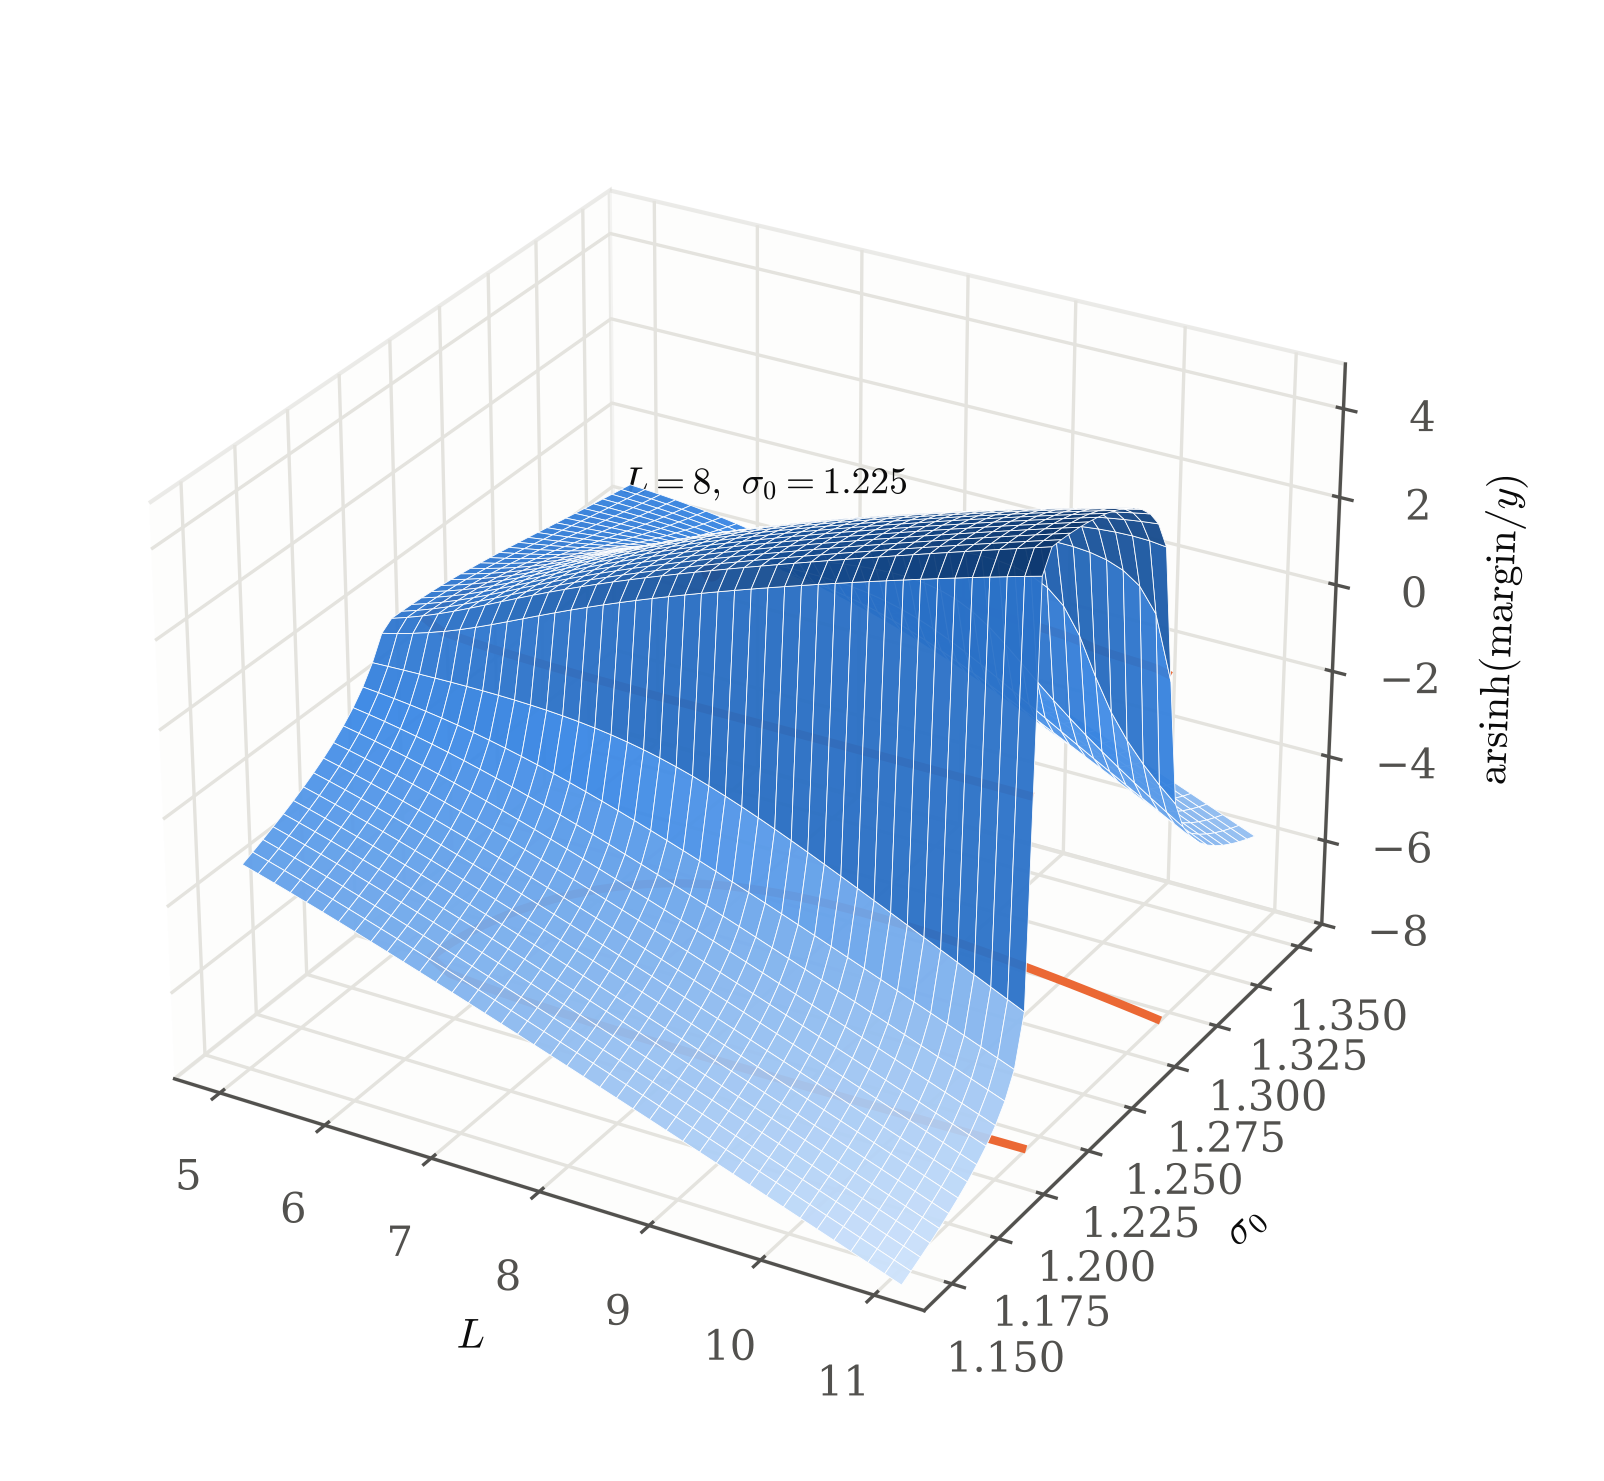
\includegraphics[width=0.78\textwidth]{fig_margin.png}
\caption{The certified quantity $(\Psi-R-2E-T-Z)/y$ of Proposition~\ref{prop:criterion} under $\Hyp(7/8)$ at $\log q=22$, with $y$ chosen so that $ye^L=(2\log q)^8$, as a function of $L$ and $\sigma_0$ (vertical scale $\operatorname{arsinh}$). The orange curve on the floor is the boundary of the region where the quantity is positive; the point used in the proof is marked.}
\label{fig:margin}
\end{figure}

\subsection{The sum over zeros}

\begin{lemma}\label{lem:zeros}
Assume that every zero of $L(s,\chi)$ satisfies $1-B\le\beta\le B$, where $\tfrac12\le B<1$, let $\chi$ be odd, and let $\sigma_0>1$. Put
\[
h_0(\sigma_0)=\frac12\psi\Bigl(\frac{\sigma_0+1}2\Bigr)-\frac12\log\pi-\frac{\zeta'}{\zeta}(\sigma_0),\qquad M=\max\Bigl(4\bigl(\sigma_0-\tfrac12\bigr),\frac1{\sigma_0-B}\Bigr).
\]
Then for $L>0$ and $y>1$,
\[
\Bigl|\sum_\rho y^\rho F(\rho)\Bigr|\ \le\ Z:=\frac4L\Bigl(\frac12\log q+h_0(\sigma_0)\Bigr)\Bigl(y^B\cosh^2\frac{BL}2\cdot M+y^{1/2}\cosh^2\frac L4\cdot\frac{\sigma_0}{(1-B)^2}\Bigr).
\]
\end{lemma}

\begin{proof}
Put $w(\rho)=(\sigma_0-\beta)/((\sigma_0-\beta)^2+\gamma^2)>0$. For every $R\ge\max\bigl((\sigma_0-\beta)/\beta^2,\,1/(\sigma_0-\beta)\bigr)$ we have
\[
(\sigma_0-\beta)^2+\gamma^2\le R(\sigma_0-\beta)\beta^2+R(\sigma_0-\beta)\gamma^2,\quad\text{that is,}\quad \frac1{|\rho|^2}\le R\,w(\rho).
\]
If $\tfrac12\le\beta\le B$, then $(\sigma_0-\beta)/\beta^2\le4(\sigma_0-\frac12)$ and $1/(\sigma_0-\beta)\le1/(\sigma_0-B)$, so $R=M$ is allowed; also $y^\beta\cosh^2(\beta L/2)\le y^B\cosh^2(BL/2)$. If $1-B\le\beta<\tfrac12$, then $(\sigma_0-\beta)/\beta^2\le\sigma_0/(1-B)^2$ and $1/(\sigma_0-\beta)\le 1/(\sigma_0-\frac12)<2\le\sigma_0/(1-B)^2$, because $(1-B)^2\le\frac14$ and $\sigma_0>1$; so $R=\sigma_0/(1-B)^2$ is allowed, and $y^\beta\cosh^2(\beta L/2)\le y^{1/2}\cosh^2(L/4)$. Since $|y^\rho F(\rho)|\le 4y^\beta\cosh^2(\beta L/2)/(L|\rho|^2)$, each zero contributes at most $\frac4L\,w(\rho)$ times the bracket in $Z$. Summing over $\rho$ and applying Lemma~\ref{lem:hadamard} with $a=1$ proves the lemma.
\end{proof}

\section{The least split prime}\label{sec:proofA}

Write $\theta(t)=\sum_{p\le t}\log p$ and $\psi(t)=\sum_{n\le t}\Lambda(n)$ (no confusion with the digamma function will arise). We use two inequalities of Rosser and Schoenfeld \cite{RS62}:
\begin{equation}\label{eq:RS}
\theta(t)>t\Bigl(1-\frac1{\log t}\Bigr)\quad(t\ge41),\qquad \psi(t)<1.03883\,t\quad(t>0),
\end{equation}
which are \cite[(3.16)]{RS62} and \cite[Theorem 12]{RS62}.

\begin{proposition}\label{prop:criterion}
Let $\chi$ be a real, odd, primitive character modulo $q\ge3$ such that every zero of $L(s,\chi)$ satisfies $1-B\le\beta\le B$, where $\tfrac12\le B<1$. Let $L>0$, $y\ge41$ with $y>e^L$, put $Y=ye^L$, let $\sigma_0>1$, and let $Z$ be as in Lemma~\ref{lem:zeros}. Put
\begin{align*}
\Psi&=\frac yL\Bigl[\Bigl(1-\frac1{\log y}\Bigr)(e^L-1)-1.03883\,(1-e^{-L})\Bigr],&
R&=\log q\Bigl(1+\frac{2L}{\log2}\Bigr),\\
E&=1.03883\Bigl(\sqrt Y+Y^{1/3}\frac{\log Y}{\log 2}\Bigr),&
T&=\frac{\pi^2e^L}{8Ly}.
\end{align*}
If $\Psi-R-2E-T>Z$, then $\chi(p)=1$ for some prime $p\le Y$.
\end{proposition}

\begin{proof}
Suppose $\chi(p)\neq1$ for every prime $p\le Y$, and let $S=\sum_n\Lam(n)g(n)$. Since $\chi$ is real, $\chi(p)\in\{-1,0\}$ for $p\le Y$, with $\chi(p)=0$ exactly when $p\mid q$.

\emph{Upper bound for $S$.} The function $g$ vanishes outside $[ye^{-L},Y]$ and $0\le g\le1$. For $p\nmid q$ we have $\chi(p)\Lambda(p)=-\Lambda(p)$ and $\chi(p^k)\Lambda(p^k)\le\Lambda(p^k)=-\Lambda(p^k)+2\Lambda(p^k)$ for $k\ge2$; for $p\mid q$ the term is $0=-\Lambda(p^k)+\Lambda(p^k)$. Hence
\[
S\le-\sum_n\Lambda(n)g(n)+\sum_{p\mid q}\sum_{k}\Lambda(p^k)g(p^k)+2\sum_{\substack{p^k\le Y\\k\ge2}}\log p .
\]
For $p\mid q$ at most $2L/\log p+1$ powers $p^k$ lie in $[ye^{-L},Y]$, so the middle sum is at most $\sum_{p\mid q}(2L+\log p)\le 2L\omega(q)+\log q\le R$, because $\omega(q)\le\log q/\log 2$. The last sum is $\psi(Y)-\theta(Y)=\sum_{2\le k\le\log Y/\log2}\theta(Y^{1/k})$, which by \eqref{eq:RS} is at most $1.03883\sqrt Y+(\log Y/\log 2)\,1.03883\,Y^{1/3}=E$. For the first sum,
\[
\sum_n\Lambda(n)g(n)\ge\sum_p\log p\,g(p)=-\int_{ye^{-L}}^{Y}\theta(t)g'(t)\,dt=\int_y^Y\frac{\theta(t)}{Lt}\,dt-\int_{ye^{-L}}^y\frac{\theta(t)}{Lt}\,dt ,
\]
by partial summation, since $g$ is Lipschitz and vanishes at both ends, with $g'(t)=1/(Lt)$ on $(ye^{-L},y)$ and $g'(t)=-1/(Lt)$ on $(y,Y)$. By \eqref{eq:RS}, the first integral is at least $(1-1/\log y)(Y-y)/L$ and the second is at most $1.03883\,(y-ye^{-L})/L$. Therefore $\sum_n\Lambda(n)g(n)\ge\Psi$ and $S\le-\Psi+R+2E$.

\emph{Lower bound for $S$.} By Lemma~\ref{lem:triangle} and Lemma~\ref{lem:zeros},
\[
S\ge-\Bigl|\sum_\rho y^\rho F(\rho)\Bigr|-\sum_{k\ge0}y^{-1-2k}F(-1-2k)\ge-Z-\frac1L\sum_{k\ge0}\frac{(e^L/y)^{1+2k}}{(1+2k)^2}\ge-Z-T,
\]
using $F(-1-2k)\le e^{(1+2k)L}/(L(1+2k)^2)$, $e^L/y<1$ and $\sum_{k\ge0}(2k+1)^{-2}=\pi^2/8$. Comparing the two bounds gives $\Psi-R-2E-T\le Z$.
\end{proof}

\begin{proof}[Proof of Theorem~\ref{thm:A}]
Let $B\in\{7/8,11/12\}$, $k=1/(1-B)\in\{8,12\}$, $c=2$, $L=8$, and $\sigma_0=1.225$ for $B=7/8$, $\sigma_0=1.27$ for $B=11/12$. Let $q=|d|$ and $q_0=e^{22}$.

\emph{Large discriminants.} Let $q\ge q_0$ and choose $y=e^{-L}(c\log q)^k$, so that $Y=(c\log q)^k$. The character $\chi_d$ is real, odd and primitive modulo $q$, and $\Hyp(B)$ gives $1-B\le\beta\le B$. At $q=q_0$ the certified values (Appendix~\ref{app:numerics}) are $\log y=22.2735\ldots$ and $(\Psi-R-2E-T-Z)/y=7.8330\ldots$ for $B=7/8$, and $\log y=37.4102\ldots$, $(\Psi-R-2E-T-Z)/y=12.0702\ldots$ for $B=11/12$; in both cases $y\ge41$, $y>e^L$ and $h_0(\sigma_0)>0$. Figure~\ref{fig:margin} shows this quantity near the chosen parameters. We show that $(\Psi-R-2E-T-Z)/y$ does not decrease as $q$ grows; then Proposition~\ref{prop:criterion} gives $P(d)\le Y=(2\log q)^k$ for all $q\ge q_0$.

As $q$ grows, $y$ grows. The quantity $\Psi/y$ depends on $q$ only through $1-1/\log y$, which increases. Next $R/y\propto\log q/(\log q)^k$ decreases, $T/y\propto y^{-2}$ decreases, $\sqrt Y/y=e^{L/2}y^{-1/2}$ decreases, and $Y^{1/3}\log Y/y=e^{L/3}y^{-2/3}\log(e^Ly)$ decreases because $\log(e^Ly)>3/2$. In $Z/y$, the identity $(B-1)k=-1$ gives $y^{B-1}=e^{L/k}/(c\log q)$, so
\[
\Bigl(\frac12\log q+h_0\Bigr)y^{B-1}=\frac{e^{L/k}}{c}\Bigl(\frac12+\frac{h_0}{\log q}\Bigr),
\]
which decreases because $h_0>0$; and $(\frac12\log q+h_0)y^{-1/2}$ is a constant times $(\frac12t+h_0)t^{-k/2}$ with $t=\log q$, which decreases because $k/2>1$ and $h_0>0$. Hence every negative term of $(\Psi-R-2E-T-Z)/y$ decreases in absolute value and the positive term increases.

\emph{Small discriminants.} For $7\le q\le q_0$ Lemma~\ref{lem:trivial} gives $P(d)\le(q+4)/4$, and $(q+4)/4<(2\log q)^8$ throughout this range. This is checked in interval arithmetic on the $412$ intervals $[a,1.05a]$ that cover $[7,q_0]$, comparing $(1.05a+4)/4$ with $(2\log a)^8$; both sides increase, so this suffices. The same check holds with exponent $12$. Finally $P(-3)=7<(2\log3)^8$ and $P(-4)=5<(2\log4)^8$.
\end{proof}

\begin{proof}[Proof of Theorem~\ref{thm:B}]
By Corollary~\ref{cor:EP} and Theorem~\ref{thm:A}, $E(d)\ge\log(|d|/4)/\log P(d)\ge\log(|d|/4)/(k\log(2\log|d|))$. If $E(d)\le e$, then $\varphi(t)=t-\log4-ke\log(2t)\le0$ at $t=\log|d|$. The function $\varphi$ increases for $t>ke$ and tends to infinity, so $\log|d|$ is at most its largest zero $t_e$, and $N_e=e^{t_e}$. Table~\ref{tab:Ne} lists $\log_{10}N_e$ rounded up, from a certified bisection.
\end{proof}

\begin{figure}[ht]
\centering
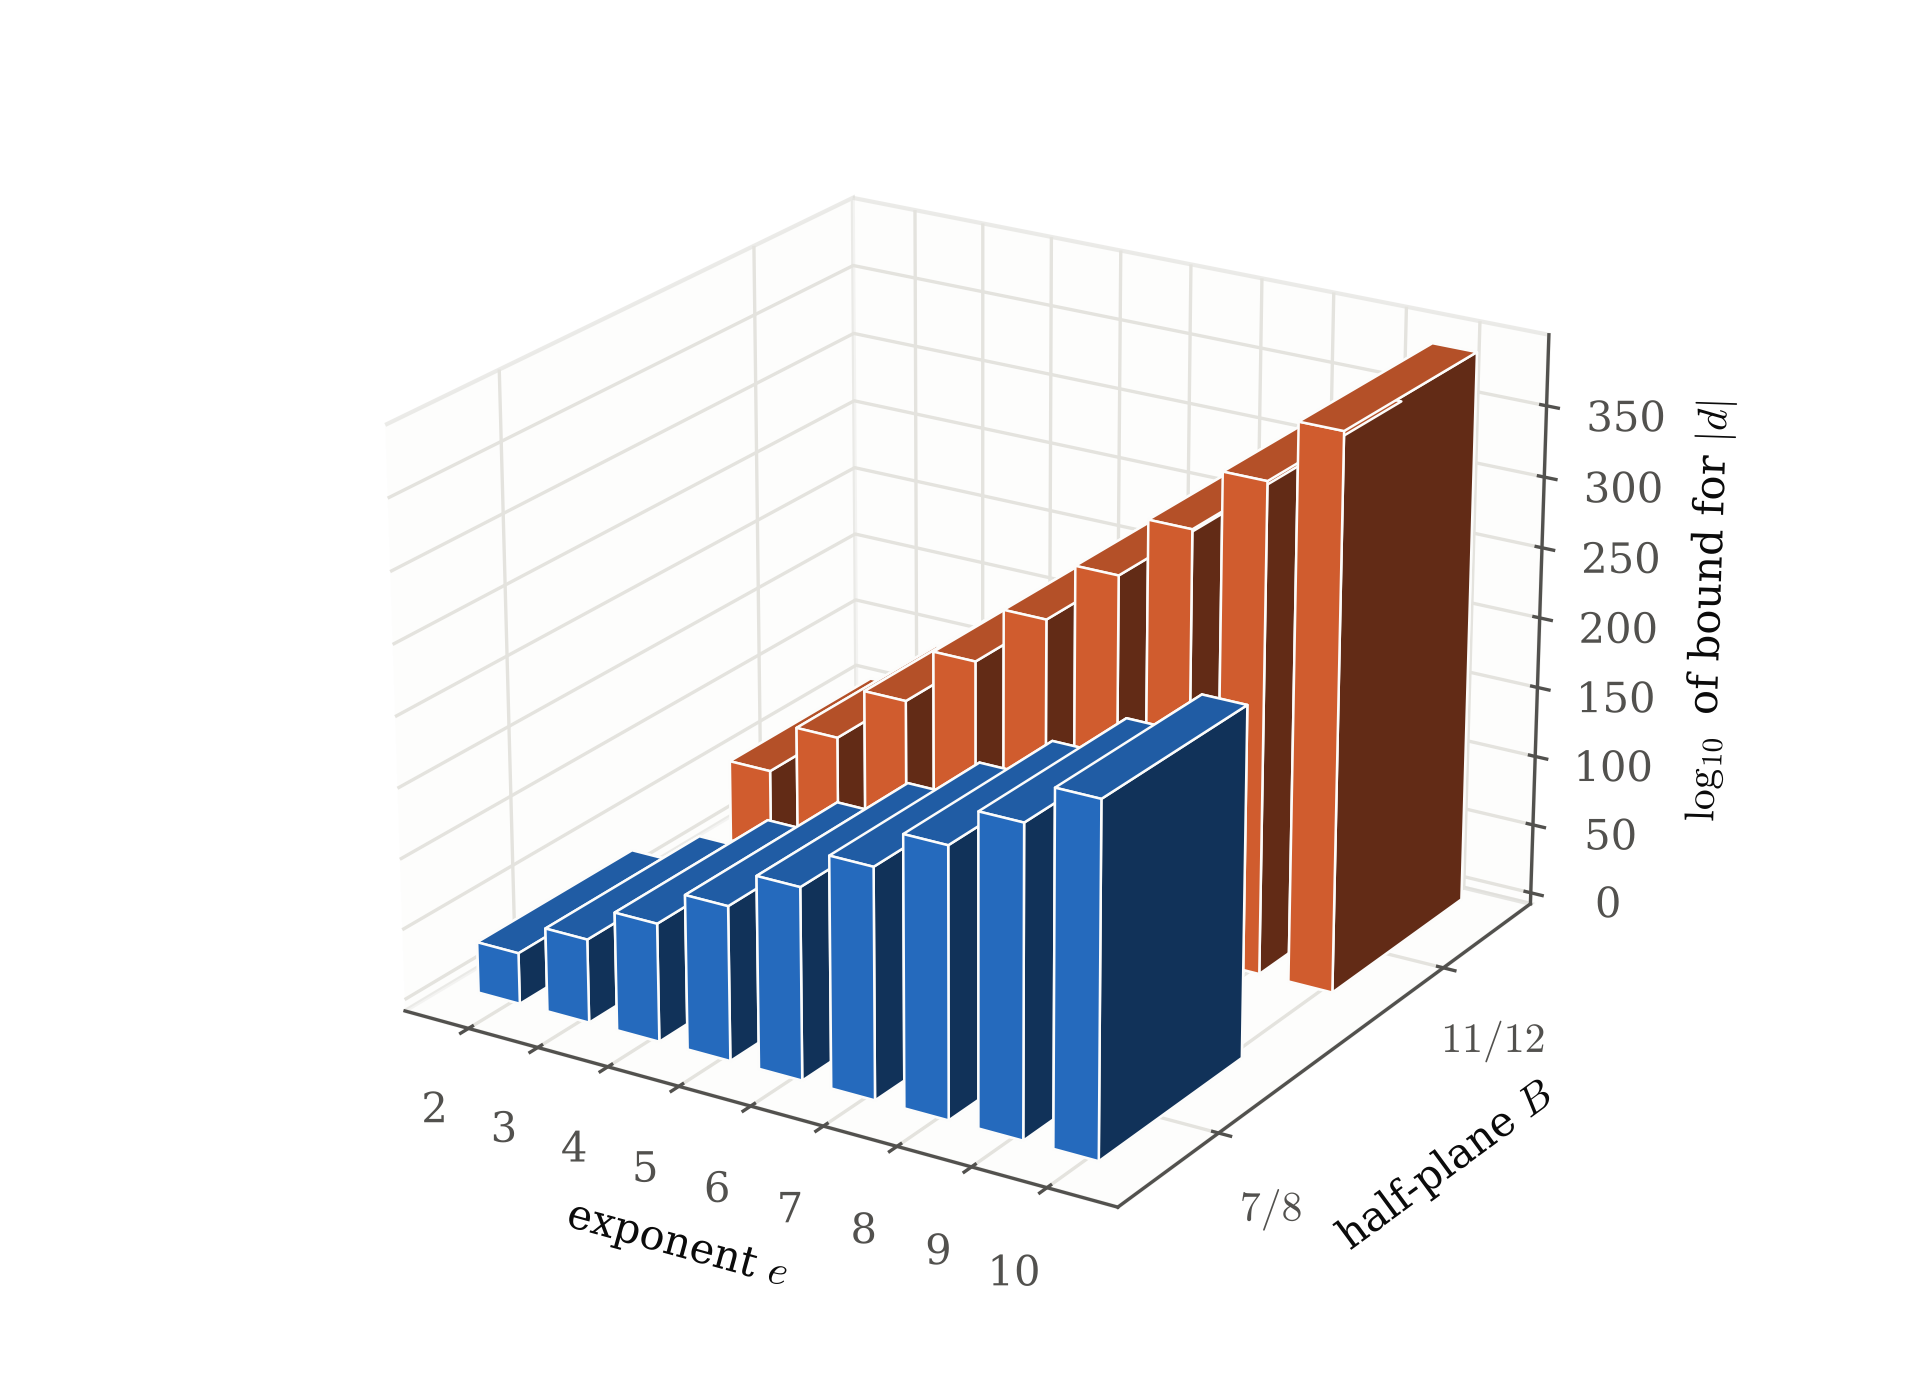
\includegraphics[width=0.74\textwidth]{fig_exponent.png}
\caption{The bounds $\log_{10}N_e$ of Theorem~\ref{thm:B}: every imaginary quadratic field whose class group has exponent at most $e$ has $|d|\le N_e$.}
\label{fig:exponent}
\end{figure}

\begin{remark}\label{rem:EKN}
Elsenhans, Kl\"uners and Nicolae show that if $L(s,\chi_d)\neq0$ for $1-1/(4\log|d|)\le s<1$ for every $|d|>e^{11.2}$, then $h(d)>0.655\sqrt{|d|}/(\pi e\log|d|)$ for those $d$, and with this bound their computation finds every field with $E(d)\in\{2,4,8\}$ \cite{EKN20}. Since $1-1/(4\cdot 11.2)>11/12$, the condition follows from $\Hyp(11/12)$. Their lists of fields of exponent $4$ and $8$ are therefore complete under $\Hyp(11/12)$, and for exponent $2$ their list agrees with Theorem~\ref{thm:C}.
\end{remark}

\section{A lower bound for \texorpdfstring{$L(1,\chi)$}{L(1,chi)}}\label{sec:L1}

The proof of Theorem~\ref{thm:C} needs $h(d)$ to be large for $|d|>2^{40}$. Theorem~\ref{thm:B} alone is not enough: under $\Hyp(7/8)$, $E(d)\le2$ gives only $|d|\le10^{36.15}$, far beyond the reach of a computation. We prove instead a lower bound for $L(1,\chi)$ of Littlewood's shape $1/\log\log q$. The notation is that of Section~\ref{sec:explicit}.

\begin{lemma}\label{lem:explicit2}
For $x>1$ and $u\ge0$,
\begin{multline*}
\sum_{n\le x}\frac{\Lam(n)}{n^{1+u}}\log\frac xn
=-\frac{L'}{L}(1+u,\chi)\log x-\Bigl(\frac{L'}{L}\Bigr)'(1+u,\chi)\\
-\sum_\rho\frac{x^{\rho-1-u}}{(\rho-1-u)^2}
-\sum_{k\ge0}\frac{x^{-2k-a-1-u}}{(2k+a+1+u)^2},
\end{multline*}
and both sums converge absolutely.
\end{lemma}

\begin{proof}
Put $s=1+u$. For $t>0$ and $c>0$, $\frac1{2\pi i}\int_{(c)}t^ww^{-2}\,dw=\max(\log t,0)$ with absolute convergence, so termwise integration gives
\[
\sum_{n\le x}\frac{\Lam(n)}{n^{s}}\log\frac xn=\frac1{2\pi i}\int_{(1)}\Bigl(-\frac{L'}{L}(s+w,\chi)\Bigr)\frac{x^w}{w^2}\,dw .
\]
The integrand has a double pole at $w=0$ with residue $-\frac{L'}{L}(s,\chi)\log x-(\frac{L'}{L})'(s,\chi)$, a pole at $w=\rho-s$ with residue $-x^{\rho-s}/(\rho-s)^2$ for each zero counted with multiplicity, and a pole at $w=-2k-a-s$ with residue $-x^{-2k-a-s}/(2k+a+s)^2$. Moving the line of integration to the left (Appendix~\ref{app:contour}) proves the formula. Absolute convergence follows from $|\rho-s|\ge|\rho-1|\gg|\rho|$.\footnote{The square in the kernel $x^w/w^2$ is what makes the sum over zeros converge absolutely without truncation in height.}
\end{proof}

Here $\log L(s,\chi)=\sum_{n\ge2}\Lam(n)n^{-s}/\log n$ for $\Re s>1$, continued along the real segment to $s=1$; this is possible because $L(1+u,\chi)\neq0$ for $u\ge0$.

\begin{proposition}\label{prop:integrated}
For $x>1$ let $V(x)=\sum_{2\le n\le x}\frac{\Lam(n)}{n\log n}\log\frac xn$. Then
\[
V(x)=\log L(1,\chi)\log x+\frac{L'}{L}(1,\chi)-\sum_\rho I_\rho(x)-T_1(x),
\]
where
\[
|I_\rho(x)|\le\frac{x^{\beta-1}}{|\rho-1|^2\log x},\qquad|T_1(x)|\le\frac{\pi^2}{8x\log x}.
\]
\end{proposition}

\begin{proof}
Integrate Lemma~\ref{lem:explicit2} over $u\in[0,\infty)$. On the left, $\int_0^\infty n^{-1-u}\,du=1/(n\log n)$ gives $V(x)$. On the right, $\int_0^\infty-\frac{L'}{L}(1+u,\chi)\,du=\log L(1,\chi)$ and $\int_0^\infty-(\frac{L'}{L})'(1+u,\chi)\,du=\frac{L'}{L}(1,\chi)$, since $\log L(1+u,\chi)$ and $\frac{L'}{L}(1+u,\chi)$ tend to $0$. The zero term is $I_\rho(x)=\int_0^\infty x^{\rho-1-u}(\rho-1-u)^{-2}\,du$; since $|\rho-1-u|^2=(1-\beta+u)^2+\gamma^2\ge|\rho-1|^2$,
\[
|I_\rho(x)|\le\frac{x^{\beta-1}}{|\rho-1|^2}\int_0^\infty x^{-u}\,du=\frac{x^{\beta-1}}{|\rho-1|^2\log x}.
\]
In the same way the $k$-th trivial term is at most $x^{-2k-a-1}/((2k+a+1)^2\log x)$, and $\sum_{k\ge0}(2k+a+1)^{-2}\le\pi^2/8$. The interchanges of sum and integral are justified by these bounds and $\sum_\rho|\rho-1|^{-2}<\infty$.
\end{proof}

\begin{corollary}\label{cor:difference}
Let $1<y<x$, $\ell=\log(x/y)$, and let $w(n)=1$ for $n\le y$, $w(n)=\log(x/n)/\ell$ for $y<n\le x$, $w(n)=0$ for $n>x$. Then
\[
\log L(1,\chi)=\sum_{n\ge2}\frac{\Lam(n)w(n)}{n\log n}+\vartheta\,\mathcal E,\qquad|\vartheta|\le1,
\]
where, with $\beta^*=\sup_\rho\beta$,
\[
\mathcal E=\frac1\ell\Bigl[\Bigl(\frac{x^{\beta^*-1}}{\log x}+\frac{y^{\beta^*-1}}{\log y}\Bigr)\sum_\rho\frac1{|\rho-1|^2}+\frac{\pi^2}{8}\Bigl(\frac1{x\log x}+\frac1{y\log y}\Bigr)\Bigr].
\]
\end{corollary}

\begin{proof}
For $n\le y$, $\log(x/n)-\log(y/n)=\ell$, and for $y<n\le x$ only $\log(x/n)$ occurs, so $V(x)-V(y)=\ell\sum\Lam(n)w(n)/(n\log n)$. Subtracting the formulas of Proposition~\ref{prop:integrated} at $x$ and $y$ removes $\frac{L'}{L}(1,\chi)$, and the bounds there give the claim.
\end{proof}

\begin{lemma}\label{lem:zerosum}
If every zero of $L(s,\chi)$ has $\beta\le B$, where $\tfrac12\le B<1$, then for every $u>0$
\[
\sum_\rho\frac1{|\rho-1|^2}\le S(q,u,B):=\frac{1+u-B}{(1-B)^2}\Bigl(\frac12\log\frac q\pi+\frac12\psi\Bigl(1+\frac u2\Bigr)-\frac{\zeta'}{\zeta}(1+u)\Bigr).
\]
\end{lemma}

\begin{proof}
Let $\sigma=1+u$. Since $\sigma-\beta\ge1-\beta>0$, we have $|\sigma-\rho|\le\frac{\sigma-\beta}{1-\beta}|1-\rho|$, hence
\[
\frac1{|1-\rho|^2}\le\frac{\sigma-\beta}{(1-\beta)^2}\cdot\frac{\sigma-\beta}{|\sigma-\rho|^2}.
\]
The function $\beta\mapsto(\sigma-\beta)/(1-\beta)^2$ has derivative $(2\sigma-1-\beta)/(1-\beta)^3>0$ on $(-\infty,1)$, so it is at most $(\sigma-B)/(1-B)^2$. Sum over $\rho$ and apply Lemma~\ref{lem:hadamard}, using $\psi((\sigma+a)/2)\le\psi(1+u/2)$.
\end{proof}

Let $B_1=0.2614972128\ldots$ be Mertens' constant and $\gamma$ Euler's constant, and put
\[
G(y)=\sum_{p\le y}\Bigl(\frac1p-\log\Bigl(1+\frac1p\Bigr)\Bigr),\qquad W=\frac1\ell\int_{\log y}^{\log x}\Bigl(\log v+B_1+\frac1{2v^2}\Bigr)dv .
\]
The terms of $G$ are positive, so $G$ increases.

\begin{lemma}\label{lem:primes}
Let $286\le y<x$, $\ell=\log(x/y)$, and let $\mathcal M$ be the sum in Corollary~\ref{cor:difference}. Then
\[
-W+G(y)-\frac3{\sqrt y}\le\Re\mathcal M\le W+\gamma-B_1+\frac3{\sqrt y}.
\]
\end{lemma}

\begin{proof}
Since $\Lambda(p^k)/(p^k\log p^k)=1/(kp^k)$ and $w(p^k)=1$ for $p^k\le y$,
\[
\mathcal M=\sum_{p\le y}-\log\Bigl(1-\frac{\chi(p)}p\Bigr)+\sum_{y<p\le x}\frac{\chi(p)w(p)}p+\mathcal R,
\]
where
\[
\mathcal R=\sum_{\substack{p\le y,\ k\ge2\\ p^k>y}}\frac{\chi(p)^k(w(p^k)-1)}{kp^k}+\sum_{\substack{p>y\\ k\ge2}}\frac{\chi(p)^kw(p^k)}{kp^k}.
\]
As $0\le w\le1$, $|\mathcal R|\le\frac12\sum_p\sum_{k\ge2,\,p^k>y}p^{-k}$. For fixed $p$ let $k_0$ be the least $k\ge2$ with $p^k>y$; the inner sum is at most $p^{-k_0}p/(p-1)\le2p^{-k_0}$. If $p\le\sqrt y$ then $p^{-k_0}<1/y$, and there are at most $\sqrt y$ such primes; if $p>\sqrt y$ then $k_0=2$. Hence $|\mathcal R|\le1/\sqrt y+\sum_{m>\sqrt y}m^{-2}\le1/\sqrt y+1/(\sqrt y-1)\le3/\sqrt y$.

For the lower bound, $-\log|1-\chi(p)/p|\ge-\log(1+1/p)$ and $\Re\chi(p)w(p)/p\ge-w(p)/p$. With $P(t)=\sum_{p\le t}1/p$, partial summation gives the identity
\[
\sum_{p\le y}\frac1p+\sum_{y<p\le x}\frac{\log(x/p)}{\ell\,p}=\frac1\ell\int_y^xP(t)\,\frac{dt}t ,
\]
and Rosser and Schoenfeld \cite[(3.18)]{RS62} give $P(t)<\log\log t+B_1+1/(2\log^2t)$ for $t\ge286$. With $v=\log t$ the right-hand side is at most $W$, which proves the lower bound. For the upper bound we use $-\log|1-\chi(p)/p|\le-\log(1-1/p)$ and Mertens' identity
\[
\sum_p\Bigl(-\log\Bigl(1-\frac1p\Bigr)-\frac1p\Bigr)=\gamma-B_1,
\]
whose terms are positive, so that $\sum_{p\le y}-\log(1-1/p)\le P(y)+\gamma-B_1$.\footnote{The identity follows from Mertens' theorems $\prod_{p\le t}(1-1/p)^{-1}\sim e^\gamma\log t$ and $\sum_{p\le t}1/p=\log\log t+B_1+o(1)$ by taking logarithms \cite[Theorem 2.7]{MV07}.} The rest is as before.
\end{proof}

\begin{theorem}\label{thm:uniform}
Assume $\Hyp(B)$ with $\tfrac12\le B<1$ and put $k=1/(1-B)$. Let $q_0\ge3$, $y_0\ge10^6$, $\ell>0$, $u>0$, and suppose that
$c_0=\frac12\psi(1+\frac u2)-\frac12\log\pi-\frac{\zeta'}{\zeta}(1+u)>0$. Let
\[
E_0=\frac1\ell\Bigl[\Bigl(\frac{x_0^{B-1}}{\log x_0}+\frac{y_0^{B-1}}{\log y_0}\Bigr)S(q_0,u,B)+\frac{\pi^2}{8}\Bigl(\frac1{x_0\log x_0}+\frac1{y_0\log y_0}\Bigr)\Bigr],\qquad x_0=e^\ell y_0,
\]
$\kappa_0=\log y_0+\ell/2-k\log\log q_0$, and
\[
C_-=\exp\Bigl(G(10^6)-B_1-\frac1{2\log^2y_0}-\frac3{\sqrt{y_0}}-E_0\Bigr).
\]
Then every primitive character $\chi$ of conductor $q\ge q_0$ satisfies $|L(1,\chi)|\ge C_-/(k\log\log q+\kappa_0)$.
\end{theorem}

\begin{proof}
Take $y=y_0(\log q/\log q_0)^k$ and $x=e^\ell y$ in Corollary~\ref{cor:difference}, so that $y\ge y_0$ and $\log y+\ell/2=k\log\log q+\kappa_0$. Under $\Hyp(B)$, $\beta^*\le B$, and Lemma~\ref{lem:zerosum} bounds the zero sum by $S(q,u,B)=A(\frac12\log q+c_0)$ with $A=(1+u-B)/(1-B)^2$. Since $(B-1)k=-1$,
\[
y^{B-1}S(q,u,B)=y_0^{B-1}\log q_0\cdot A\Bigl(\frac12+\frac{c_0}{\log q}\Bigr),
\]
which decreases in $q$ because $c_0>0$; the same holds with $x$ in place of $y$, and the remaining factors of $\mathcal E$ decrease too. Hence $\mathcal E\le E_0$. For the prime sum, concavity of $\log$ gives $\ell^{-1}\int_{\log y}^{\log x}\log v\,dv\le\log(\log y+\ell/2)$, and $\ell^{-1}\int_{\log y}^{\log x}dv/(2v^2)\le1/(2\log^2y_0)$, so $W\le\log(k\log\log q+\kappa_0)+B_1+1/(2\log^2y_0)$. Also $G(y)\ge G(10^6)$ and $3/\sqrt y\le3/\sqrt{y_0}$. Taking real parts in Corollary~\ref{cor:difference} and inserting Lemma~\ref{lem:primes} gives $\log|L(1,\chi)|\ge-W+G(y)-3/\sqrt y-E_0$, and exponentiating proves the theorem.
\end{proof}

For a fundamental $d<-4$ the class number formula reads $h(d)=\sqrt{|d|}\,L(1,\chi_d)/\pi$ \cite[Chapter 6]{Dav80}.

\begin{corollary}\label{cor:h}
Let $d<-2^{40}$ be fundamental. Under $\Hyp(7/8)$,
\[
h(d)\ \ge\ \frac{0.72554\sqrt{|d|}}{\pi\,(8\log\log|d|-4.15398)}\ \ge\ 10\,798.96 ,
\]
and under $\Hyp(11/12)$, $h(d)\ge 0.71408\sqrt{|d|}/(\pi(12\log\log|d|-8.55734))\ge7\,612.06$.
\end{corollary}

\begin{proof}
Apply Theorem~\ref{thm:uniform} with $q_0=2^{40}$ and, for $B=7/8$, $y_0=5\cdot10^6$, $\ell=14$, $u=1/10$; for $B=11/12$, $y_0=1.8\cdot10^9$, $\ell=20$, $u=0.08$. The certified constants are in Appendix~\ref{app:numerics}. The function $f(q)=C_-\sqrt q/(\pi(k\log\log q+\kappa_0))$ increases for $q\ge2^{40}$, since $\frac{d}{dq}\log f(q)=\frac1{2q}-\frac{k}{q\log q\,(k\log\log q+\kappa_0)}>0$ there, and $f(2^{40})$ is the stated number.
\end{proof}

\section{Class groups of exponent two}\label{sec:two}

\begin{proof}[Proof of Theorem~\ref{thm:C}]
We first determine the fundamental discriminants $d$ with $E(d)\le2$, in three ranges, and then pass to all discriminants.

\emph{$|d|\le10^6$.} For every discriminant $D$ with $|D|\le10^6$ we listed the primitive reduced forms $(a,b,c)$, using $a\le\sqrt{|D|/3}$, and checked by Lemma~\ref{lem:ambiguous} whether all of them have order at most $2$. Exactly $101$ discriminants pass, $65$ of them fundamental, the largest $|D|$ being $7392$ and the largest fundamental $|d|$ being $5460$.\footnote{For $|D|\le10^6$ the enumeration covers non-fundamental discriminants as well, which gives an independent check of the reduction carried out below.}

\emph{$10^6<|d|\le2^{40}$.} If $E(d)\le2$, Lemma~\ref{lem:order} with $c=2$ shows that no prime $p$ with $4p^2<|d|$ splits in $K$. In particular $2$ does not split, so $d\not\equiv1\pmod8$: either $d=-q$ with $q\equiv3\pmod 8$, or $d=-4m$ with $m\equiv1,2\pmod4$. For every such $q$, respectively $m$, in the range we tested the condition $\chi_d(p)\neq1$ for the odd primes $p<1000$ with $4p^2<|d|$. A wheel modulo $8\cdot3\cdot5\cdots23$, respectively $4\cdot3\cdot5\cdots23$, discards the residue classes that fail at some $p\le23$; this leaves $1\,088\,640$ classes in each case and about $1.34\cdot10^9$ values of $q$, respectively $m$, to test. None passes. Squarefreeness was not used, so the conclusion covers every fundamental $d$ in the range.\footnote{This range is also covered by the unconditional tabulation of the class groups of imaginary quadratic fields with $|d|<2^{40}$ by Mosunov and Jacobson \cite{MJ16}; the sieve above does not use it.}

\emph{$|d|>2^{40}$.} Suppose $E(d)\le2$, so that $h(d)=2^{\omega(d)-1}$. Let $t=15$ under $\Hyp(7/8)$ and $t=14$ under $\Hyp(11/12)$. If $\omega(d)<t$, then $h(d)\le2^{t-2}$, which is $8192<10\,798.96$, respectively $4096<7\,612.06$, contradicting Corollary~\ref{cor:h}. If $\omega(d)=s\ge t$, then $|d|\ge p_s\#$, the product of the first $s$ primes, and $p_s\#\ge p_t\#>2^{40}$. Let $f$ be the increasing function of the proof of Corollary~\ref{cor:h}. We claim $f(p_s\#)>2^{s-1}$ for all $s\ge t$, which contradicts $h(d)\ge f(|d|)\ge f(p_s\#)$. For $s=t$ the certified values are $f(p_{15}\#)=7.088\ldots\cdot10^6>2^{14}$ and $f(p_{14}\#)=7.468\ldots\cdot10^5>2^{13}$ in the two cases. For the step from $s$ to $s+1$, write $q=p_s\#$ and $p=p_{s+1}\le q$. Then $\log\log(qp)\le\log(2\log q)=\log\log q+\log2$, so with $A_q=k\log\log q+\kappa_0$,
\[
\frac{f(qp)}{f(q)}\ \ge\ \sqrt p\,\frac{A_q}{A_q+k\log2}\ \ge\ \sqrt{p_{t+1}}\,\frac{A_{2^{40}}}{A_{2^{40}}+k\log2}\ \ge\ 2,
\]
because $A_q\ge A_{2^{40}}>0$ for $q>2^{40}$, the factor $A/(A+k\log2)$ increases with $A$, and $p\ge p_{t+1}$, which is $p_{16}=53$, respectively $p_{15}=47$; the certified values $A_{2^{40}}=22.42\ldots$, respectively $31.30\ldots$, give $\sqrt{p_{t+1}}\,A_{2^{40}}/(A_{2^{40}}+k\log 2)\ge2$ in both cases. Hence $f(p_{s+1}\#)\ge2f(p_s\#)>2^s$.

So the fundamental discriminants with $E(d)\le2$ are the $65$ found in the first range.

\emph{Non-fundamental discriminants.} Let $D=f^2d$ with $f>1$ and $d$ fundamental, and suppose $C(D)$ has exponent at most $2$. The natural map $C(D)\to\Cl(d)$ is surjective \cite[\S7]{Cox13}, so $E(d)\le2$ and $d$ is one of the $65$. By the class number formula for orders \cite[Theorem 7.24]{Cox13},
\[
h(D)=\frac{h(d)\,f}{u}\prod_{p\mid f}\Bigl(1-\frac{\chi_d(p)}p\Bigr),\qquad u=[\mathcal O_K^\times:\mathcal O^\times]\in\{1,2,3\},
\]
with $u=3$ only for $d=-3$ and $u=2$ only for $d=-4$. By \eqref{eq:genus}, $h(D)=2^{\mu(D)-1}$ and $h(d)=2^{\omega(d)-1}$. Every odd prime dividing $D$ divides $d$ or $f$, and comparing the definition of $\mu$ in the cases $2\nmid D$, $2\mid f$, $2\mid d$ shows $\mu(D)\le\omega(d)+\omega(f)+1$. Since $\prod_{p\mid f}(1-\chi_d(p)/p)\ge\prod_{p\mid f}(1-1/p)$, we get
\[
\frac{\varphi(f)}{3}\le\frac{h(D)}{h(d)}\le2^{\omega(f)+1},\qquad\text{so}\qquad \prod_{p^a\parallel f}\frac{\varphi(p^a)}{2}\le6 .
\]
Each factor $\varphi(p^a)/2=p^{a-1}(p-1)/2$ is at least $1$, except $\varphi(2)/2=\frac12$, so each factor is at most $12$. This forces $p\le23$ (for $p\ge29$ the factor is at least $14$), and $2^a\mid f$ with $a\le5$, $3^a$ with $a\le3$, $5^a$ with $a\le2$, and $a\le1$ for $7\le p\le23$. Hence $f$ divides $F=2^5\cdot3^3\cdot5^2\cdot7\cdot11\cdot13\cdot17\cdot19\cdot23$, which has $4608$ divisors. For each of the $65$ fundamental $d$ and each divisor $f$ of $F$ we evaluated $h(D)$ by the class number formula and compared it with $2^{\mu(D)-1}$. Equality holds for exactly $36$ pairs with $f>1$; together with the $65$ fundamental discriminants they are the $101$ discriminants found in the first range, all with $|D|\le7392$.
\end{proof}

\begin{proof}[Proof of Corollary~\ref{cor:idoneal}]
By Grube's theorem, in the form of \cite[Theorem 3.22 and Proposition 3.24]{Cox13}, $n$ is idoneal if and only if $h(-4n)=2^{\mu(-4n)-1}$, that is, by \eqref{eq:genus}, if and only if $C(-4n)$ has exponent at most $2$. The discriminants $D\equiv0\pmod4$ among the $101$ of Theorem~\ref{thm:C} are $-4n$ for exactly the $65$ numbers listed.
\end{proof}

\begin{figure}[ht]
\centering
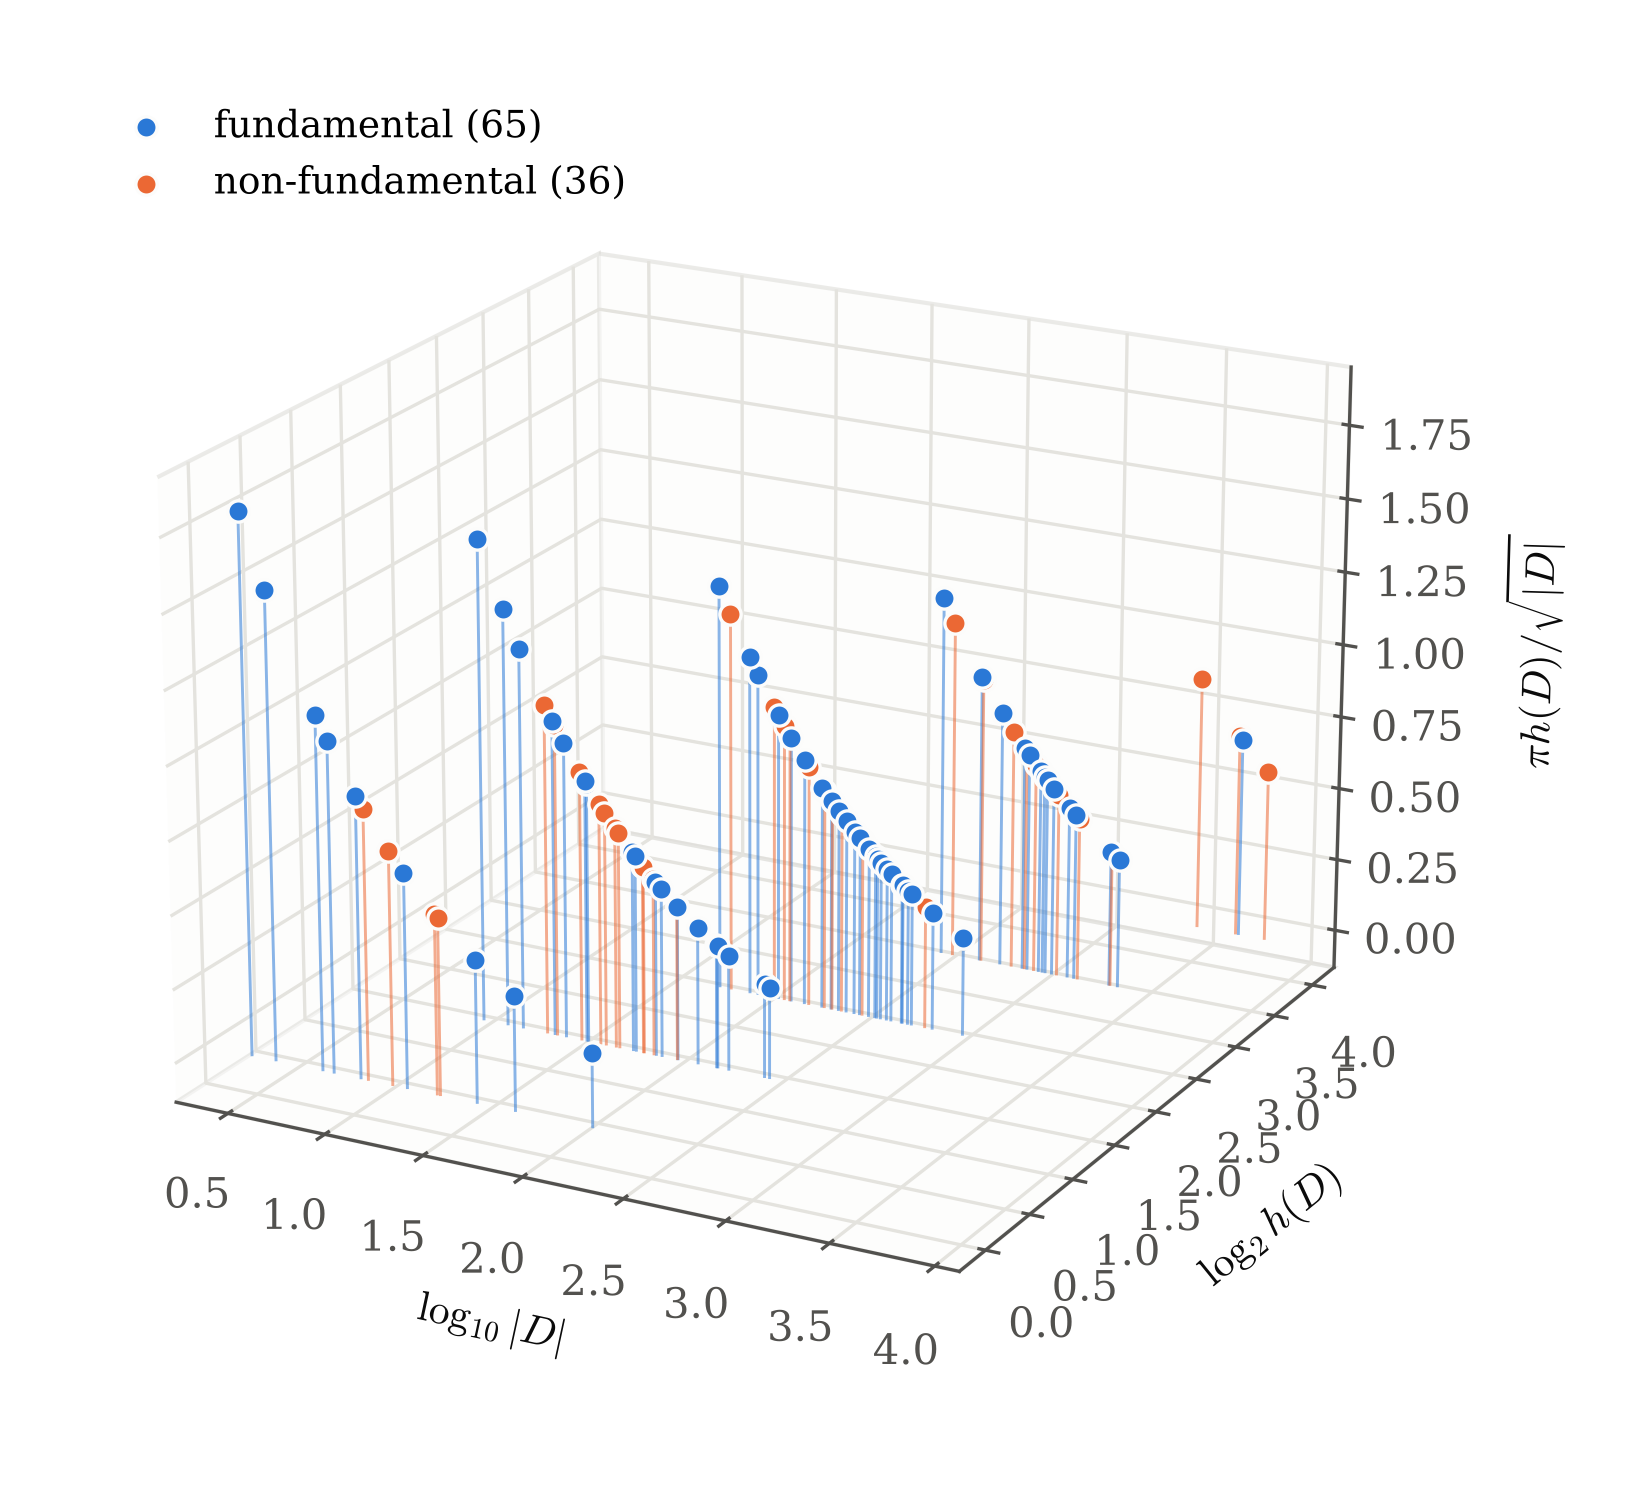
\includegraphics[width=0.74\textwidth]{fig_exptwo.png}
\caption{The $101$ discriminants of Theorem~\ref{thm:C}: $\log_{10}|D|$, $\log_2h(D)$ and $\pi h(D)/\sqrt{|D|}$, which is $L(1,\chi_d)$ for fundamental $d<-4$. The fields of exponent two have small $L(1,\chi_d)$, because every small prime is inert or ramified; this is the tension that Corollary~\ref{cor:h} resolves.}
\label{fig:exptwo}
\end{figure}

\section{Concluding remarks}\label{sec:remarks}

The exponent $k=1/(1-B)$ in Theorems~\ref{thm:A} and~\ref{thm:B} is the only place where the width of the zero-free region enters. Under the generalised Riemann hypothesis the same argument has $k=2$. Any improvement of the half-plane, or a zero-density estimate near $\Re s=B$, improves the constants at once. The method uses only the real character $\chi_d$; the same proof gives, for every real primitive character of conductor $q$, a prime $p\le(2\log q)^{k}$ with $\chi(p)=1$ when $\chi$ is odd. The half-plane $\Re s>7/8$ also yields the P\'olya--Vinogradov inequality with $\log\log q$ \cite{BhaPV}, and explicit prime computations of the kind used here underlie the author's bound for Lehmer's totient problem \cite{BhaLehmer}. Questions about the exponent of a finitely generated group arise in a different setting in the author's work on hyperbolic groups \cite{Bha22}.

Without a hypothesis on zeros, at most one fundamental discriminant is missing from Theorem~\ref{thm:C} \cite{Wei73}, and if it exists it has $|d|>2^{40}$ by the sieve of Section~\ref{sec:two}.\footnote{The sieve uses only Lemma~\ref{lem:order}, so this part is unconditional.} A refereed proof of $\Hyp(B)$ for any $B<1$ would remove the exception and make Theorems~\ref{thm:A}, \ref{thm:B} and~\ref{thm:C} unconditional, with $k=1/(1-B)$ in place of $8$ or $12$ after the certification of Appendix~\ref{app:numerics} is repeated.

\appendix

\section{The contour shifts}\label{app:contour}

We justify the shifts of contour in Lemmas~\ref{lem:triangle} and~\ref{lem:explicit2}. In both, the integrand is $-\frac{L'}{L}(s',\chi)\Phi(s')$ with $s'$ the argument of $L$: $\Phi(s')=y^{s'}F(s')$ in Lemma~\ref{lem:triangle}, and $\Phi(s')=x^{s'-s}/(s'-s)^2$ with $s=1+u$ in Lemma~\ref{lem:explicit2}. In both cases there are $\theta>1$ and $C$ such that
\begin{equation}\label{eq:kernel}
|\Phi(\sigma+it)|\le C\,\theta^{\sigma}\,(1+|t|)^{-2}\qquad(\sigma\le2,\ |\sigma+it-s_*|\ge1),
\end{equation}
where $s_*=0$, respectively $s_*=s$: take $\theta=ye^{-L}$ for $\sigma\le0$ and $\theta=y$ for $0\le\sigma\le2$ in the first case, since $|F(\sigma+it)|\le4\cosh^2(\sigma L/2)/(L|\sigma+it|^2)\le 4e^{|\sigma|L}/(L|\sigma+it|^2)$; and $\theta=x$ in the second.\footnote{In the first case two values of $\theta$ are used on the two sides of $\sigma=0$; on the left of the contour only $\theta=ye^{-L}>1$ matters.} We use three facts \cite[Chapters 12, 16, 17 and 19]{Dav80}, together with $|\frac{L'}{L}(\sigma+it,\chi)|\le-\frac{\zeta'}{\zeta}(2)$ for $\sigma\ge2$.
\begin{enumerate}[label=(\arabic*)]
\item For each $j\ge2$ there is $T_j\in[j,j+1]$ such that $|\frac{L'}{L}(\sigma\pm iT_j,\chi)|\ll\log^2(qT_j)$ uniformly for $-1\le\sigma\le2$.
\item For $\sigma\le-1$ and $s'$ at distance at least $\tfrac12$ from every trivial zero, $|\frac{L'}{L}(s',\chi)|\ll\log(q|s'|)$, by the functional equation and Stirling's formula.
\item The number of zeros with $|\gamma-t|\le1$ is $O(\log(q(|t|+2)))$.
\end{enumerate}
Let $m\ge1$ and let $\mathcal R$ be the rectangle with vertices $2\pm iT_j$ and $-U_m\pm iT_j$, where $U_m=2m+a+1$, so that the left side lies midway between two trivial zeros. By the residue theorem the integral over the right side equals the sum of the residues inside $\mathcal R$ plus the integrals over the other three sides. On the horizontal sides, \eqref{eq:kernel} and (1), (2) bound the integrand by $\ll\theta^{\sigma}\log^2(q(T_j+U_m+2))/T_j^2$, so their contribution is $\ll\theta^2\log^2(q(T_j+U_m+2))/(T_j^2\log\theta)\to0$ as $j\to\infty$ with $m$ fixed. On the left side, (2) gives the bound $\ll\theta^{-U_m}\int_{-\infty}^{\infty}\log(q(U_m+|t|+2))(1+|t|)^{-2}\,dt\ll\theta^{-U_m}\log(qU_m)\to0$ as $m\to\infty$. Letting first $j\to\infty$ and then $m\to\infty$, and using (3) to see that the residues at the nontrivial zeros form an absolutely convergent series, we obtain the two formulas. In Lemma~\ref{lem:explicit2} the right side of $\mathcal R$ is the line $\Re s'=1+s$ instead of $\Re s'=2$, which changes nothing.

\section{Certified constants}\label{app:numerics}

All constants were computed with the ball arithmetic of Arb \cite{Joh17} at $256$ bits, through python-flint; every digit shown is guaranteed. The values $\zeta'/\zeta(\sigma)$ come from the Arb power series of $\zeta$, the values of $\psi$ from its digamma function, and $G(10^6)=0.181981816529021\ldots$ is a sum of $78\,498$ terms in balls. Mertens' constant was taken to fifty digits.

\begin{center}
\begin{tabular}{@{}lll@{}}
\toprule
Theorem~\ref{thm:A} & $B=7/8$ & $B=11/12$\\
\midrule
$k,\ L,\ \sigma_0,\ c,\ \log q_0$ & $8,\ 8,\ 1.225,\ 2,\ 22$ & $12,\ 8,\ 1.27,\ 2,\ 22$\\
$\log y$ at $q_0$ & $22.273517\ldots$ & $37.410276\ldots$\\
$h_0(\sigma_0)$ & $3.1316109\ldots$ & $2.4139115\ldots$\\
$M$ & $2.9$ & $3.08$\\
$\Psi/y$ & $355.64128\ldots$ & $362.40792\ldots$\\
$Z/y$ & $347.80610\ldots$ & $350.33768\ldots$\\
$(R+2E+T)/y$ & $0.0021171\ldots$ & $0.0000009\ldots$\\
$(\Psi-R-2E-T-Z)/y$ & $7.8330627\ldots$ & $12.070238\ldots$\\
\bottomrule
\end{tabular}

\medskip
\begin{tabular}{@{}lll@{}}
\toprule
Corollary~\ref{cor:h} & $B=7/8$ & $B=11/12$\\
\midrule
$q_0,\ y_0,\ \ell,\ u$ & $2^{40},\ 5\cdot10^6,\ 14,\ 0.1$ & $2^{40},\ 1.8\cdot10^9,\ 20,\ 0.08$\\
$S(q_0,u,B)$ & $323.75077\ldots$ & $587.32747\ldots$\\
$c_0$ & $8.6197489\ldots$ & $11.108462\ldots$\\
$E_0$ & $0.2378758\ldots$ & $0.2560657\ldots$\\
$\kappa_0$ & $-4.1539838\ldots$ & $-8.5573459\ldots$\\
$C_-$ & $0.7255434\ldots$ & $0.7140853\ldots$\\
$f(2^{40})$ & $10\,798.962\ldots$ & $7\,612.065\ldots$\\
$f(p_t\#)$ & $7.0888\cdot10^6$ ($t=15$) & $7.4688\cdot10^5$ ($t=14$)\\
\bottomrule
\end{tabular}
\end{center}

\section{The discriminants of exponent at most two}\label{app:list}

The $101$ discriminants of Theorem~\ref{thm:C}, given as $|D|$ and grouped by $h(D)$; the fundamental ones are in bold.

\smallskip
\noindent\textbf{$h=1$:} \textbf{3}, \textbf{4}, \textbf{7}, \textbf{8}, \textbf{11}, 12, 16, \textbf{19}, 27, 28, \textbf{43}, \textbf{67}, \textbf{163}.

\noindent\textbf{$h=2$:} \textbf{15}, \textbf{20}, \textbf{24}, 32, \textbf{35}, 36, \textbf{40}, 48, \textbf{51}, \textbf{52}, 60, 64, 72, 75, \textbf{88}, \textbf{91}, 99, 100, 112, \textbf{115}, \textbf{123}, 147, \textbf{148}, \textbf{187}, \textbf{232}, \textbf{235}, \textbf{267}, \textbf{403}, \textbf{427}.

\noindent\textbf{$h=4$:} \textbf{84}, 96, \textbf{120}, \textbf{132}, 160, \textbf{168}, 180, 192, \textbf{195}, \textbf{228}, 240, \textbf{280}, 288, \textbf{312}, 315, \textbf{340}, 352, \textbf{372}, \textbf{408}, \textbf{435}, 448, \textbf{483}, \textbf{520}, \textbf{532}, \textbf{555}, \textbf{595}, \textbf{627}, \textbf{708}, \textbf{715}, \textbf{760}, \textbf{795}, \textbf{928}, \textbf{1012}, \textbf{1435}.

\noindent\textbf{$h=8$:} \textbf{420}, 480, \textbf{660}, 672, \textbf{840}, 960, \textbf{1092}, 1120, \textbf{1155}, 1248, \textbf{1320}, \textbf{1380}, \textbf{1428}, \textbf{1540}, \textbf{1632}, \textbf{1848}, \textbf{1995}, \textbf{2080}, \textbf{3003}, \textbf{3040}, \textbf{3315}.

\noindent\textbf{$h=16$:} \textbf{3360}, \textbf{5280}, \textbf{5460}, 7392.

\section*{Declarations}

\subsection*{Data availability}
The certification script, the sieve, the enumeration of reduced forms, the reduction of non-fundamental discriminants and their outputs are archived in \cite{Archive}. The sieve and the enumeration are C programs; the other computations use Python with Arb through python-flint and SymPy.

\subsection*{Funding}
No funding was received for conducting this study.

\subsection*{Conflict of interest}
The author has no conflicts of interest to declare that are relevant to the content of this article.

\subsection*{Ethics statement}
This study involves no human participants, animals or personal data; no ethical approval was required.

\subsection*{Use of AI tools}
Claude Code (Opus 5.5 and Fable 5.1, Anthropic), GPT-6.1 Sol and GPT-6 Astra (OpenAI) were used to write and run the programs behind the computations and to prepare the manuscript. The hypotheses $\Hyp(7/8)$ and $\Hyp(11/12)$ are results claimed in preprints of OpenAI \cite{OAI-a,OAI-b}, cited as such. The author checked every statement and is responsible for the content.

\begingroup\raggedright
\begin{thebibliography}{99}

\bibitem{Ank52} N.~C.~Ankeny, \emph{The least quadratic non residue}, Ann. of Math. (2) \textbf{55} (1952), 65--72. \doi{10.2307/1969420}

\bibitem{Bac90} E.~Bach, \emph{Explicit bounds for primality testing and related problems}, Math. Comp. \textbf{55} (1990), 355--380. \doi{10.1090/S0025-5718-1990-1023756-8}

\bibitem{Bha22} D.~Bhattacharjee, \emph{Establishing equivariant class $[\mathcal O]$ for hyperbolic groups}, Asian Res. J. Math. \textbf{18} (2022), no.~11, 362--369. \doi{10.9734/arjom/2022/v18i11615}

\bibitem{BhaLehmer} D.~Bhattacharjee, \emph{A sixteen-prime-factor bound for Lehmer's totient problem and exact prime-completion criteria}, version 1.11.0, Zenodo, 2026. \doi{10.5281/zenodo.23795673}

\bibitem{BhaPV} D.~Bhattacharjee, P.~Mandal and U.~Bhattacharya, \emph{The P\'olya--Vinogradov inequality with $\log\log q$ for every character: paper, Lean~4 library and checking programs}, version 4.1.0, Zenodo, 2026. \doi{10.5281/zenodo.23881837}

\bibitem{BK72} D.~W.~Boyd and H.~Kisilevsky, \emph{On the exponent of the ideal class groups of complex quadratic fields}, Proc. Amer. Math. Soc. \textbf{31} (1972), 433--436. \doi{10.1090/S0002-9939-1972-0289454-4}

\bibitem{Bue89} D.~A.~Buell, \emph{Binary Quadratic Forms: Classical Theory and Modern Computations}, Springer, New York, 1989. \doi{10.1007/978-1-4612-4542-1}

\bibitem{Cho34} S.~Chowla, \emph{An extension of Heilbronn's class-number theorem}, Q. J. Math. \textbf{os-5} (1934), 304--307. \doi{10.1093/qmath/os-5.1.304}

\bibitem{Cox13} D.~A.~Cox, \emph{Primes of the Form $x^2+ny^2$: Fermat, Class Field Theory, and Complex Multiplication}, 2nd ed., John Wiley \& Sons, Hoboken, 2013. \doi{10.1002/9781118400722}

\bibitem{Dav80} H.~Davenport, \emph{Multiplicative Number Theory}, 2nd ed., revised by H.~L.~Montgomery, Graduate Texts in Mathematics \textbf{74}, Springer, New York, 1980. \doi{10.1007/978-1-4757-5927-3}

\bibitem{EK82} A.~G.~Earnest and O.~H.~K\"orner, \emph{On ideal class groups of $2$-power exponent}, Proc. Amer. Math. Soc. \textbf{86} (1982), 196--198. \doi{10.1090/S0002-9939-1982-0667271-7}

\bibitem{EKN20} A.-S.~Elsenhans, J.~Kl\"uners and F.~Nicolae, \emph{Imaginary quadratic number fields with class groups of small exponent}, Acta Arith. \textbf{193} (2020), 217--233. \doi{10.4064/aa180220-20-3}

\bibitem{HB08} D.~R.~Heath-Brown, \emph{Imaginary quadratic fields with class group exponent $5$}, Forum Math. \textbf{20} (2008), 275--283. \doi{10.1515/FORUM.2008.014}

\bibitem{Joh17} F.~Johansson, \emph{Arb: efficient arbitrary-precision midpoint-radius interval arithmetic}, IEEE Trans. Comput. \textbf{66} (2017), 1281--1292. \doi{10.1109/TC.2017.2690633}

\bibitem{Kan11} E.~Kani, \emph{Idoneal numbers and some generalizations}, Ann. Sci. Math. Qu\'ebec \textbf{35} (2011), no.~2, 197--227.

\bibitem{Lit28} J.~E.~Littlewood, \emph{On the class-number of the corpus $P(\sqrt{-k})$}, Proc. London Math. Soc. (2) \textbf{27} (1928), 358--372. \doi{10.1112/plms/s2-27.1.358}

\bibitem{MJ16} A.~S.~Mosunov and M.~J.~Jacobson,~Jr., \emph{Unconditional class group tabulation of imaginary quadratic fields to $|\Delta|<2^{40}$}, Math. Comp. \textbf{85} (2016), 1983--2009. \doi{10.1090/mcom3050}

\bibitem{MV07} H.~L.~Montgomery and R.~C.~Vaughan, \emph{Multiplicative Number Theory I. Classical Theory}, Cambridge Studies in Advanced Mathematics \textbf{97}, Cambridge University Press, Cambridge, 2007. \doi{10.1017/CBO9780511618314}

\bibitem{OAI-a} OpenAI, \emph{The quasi-Riemann hypothesis: a zero-free half-plane $\Re s>7/8$}, preprint, 30 September 2026, \url{https://github.com/openai/math}, commit 4eaee87.

\bibitem{OAI-c} OpenAI, \emph{Uniform exclusion of Landau--Siegel zeros}, preprint, 1 October 2026, \url{https://github.com/openai/math}, commit 4eaee87.

\bibitem{OAI-b} OpenAI, \emph{The quasi-Riemann hypothesis}, preprint, 5 October 2026, \url{https://github.com/openai/math}, commit 4eaee87.

\bibitem{RS62} J.~B.~Rosser and L.~Schoenfeld, \emph{Approximate formulas for some functions of prime numbers}, Illinois J. Math. \textbf{6} (1962), 64--94. \doi{10.1215/ijm/1255631807}

\bibitem{Wei73} P.~J.~Weinberger, \emph{Exponents of the class groups of complex quadratic fields}, Acta Arith. \textbf{22} (1973), 117--124. \doi{10.4064/aa-22-2-117-124}

\bibitem{Archive} D.~Bhattacharjee, \emph{Split Primes and the Exponent of Imaginary Quadratic Class Groups: paper, certification script and data}, version 1.0.0, Zenodo, 2026. \doi{10.5281/zenodo.24093928}

\end{thebibliography}
\endgroup

\end{document}
